\section{EXPERIMENTS AND RESULTS}
\label{ch:results}

This chapter reports what the notebooks computed. Unless stated otherwise, every number is copied from a notebook output, and every figure is the image saved by the notebook. We first describe the setup and the data (Sections~\ref{sec:res-setup}--\ref{sec:res-leak}), then the evidence behind the preprocessing choices (Sections~\ref{sec:res-eda} and \ref{sec:res-prep}), the model comparison (Section~\ref{sec:res-models}), the two follow-up experiments (Section~\ref{sec:res-exp}), a discussion, and the limitations (Section~\ref{sec:limits}).

\subsection{Experimental setup}
\label{sec:res-setup}

The experiments use the protocol of Chapter~\ref{ch:method}: out-of-time split by issue date, 153 features after the pipeline of Section~\ref{sec:pipeline}, hyperparameters tuned with \code{TimeSeriesSplit(3)} inside the training set, metrics ROC-AUC, Gini and KS, 1,000 paired-bootstrap resamples on validation, and a single test evaluation. The seed is 42. Metrics are reported for ranking quality only; no threshold-dependent metric (accuracy, F1) is used because no decision threshold is defined for the task.

\subsection{Dataset statistics and the time structure}
\label{sec:res-data}

\paragraph{Labels.} Of 2,260,701 loans, 1,345,310 have a final label: 1,076,751 Fully Paid (80.04\%) and 268,559 Charged Off (19.96\%) among the labelled loans. Table~\ref{tab:status} shows all statuses and the share of loans with remaining principal; the finished statuses are exactly those with no outstanding principal, which supports using the statuses \code{Fully Paid} and \code{Charged Off} as final outcomes.

\begin{table}[H]
\centering
\caption{Loan statuses in the raw file and the share of loans with outstanding principal (\code{out\_prncp}$>0$).}
\label{tab:status}
\small
\begin{tabular}{lrrr}
\toprule
\textbf{loan\_status} & \textbf{Loans} & \textbf{\% of file} & \textbf{Share with principal} \\
\midrule
Fully Paid & 1,076,751 & 47.63 & 0.000 \\
Current & 878,317 & 38.85 & 0.995 \\
Charged Off & 268,559 & 11.88 & 0.000 \\
Late (31--120 days) & 21,467 & 0.95 & 0.999 \\
In Grace Period & 8,436 & 0.37 & 0.987 \\
Late (16--30 days) & 4,349 & 0.19 & 0.992 \\
Does not meet the credit policy: Fully Paid & 1,988 & 0.09 & 0.000 \\
Does not meet the credit policy: Charged Off & 761 & 0.03 & 0.000 \\
Default & 40 & 0.00 & 1.000 \\
(missing) & 33 & 0.00 & --- \\
\bottomrule
\end{tabular}
\end{table}

\paragraph{Time structure.} Table~\ref{tab:year} shows, by issue year, how many loans exist, what fraction has a final label, the default rate among labelled loans and the share of 60-month loans. The labelled fraction is 100\% for 2011--2013 and falls to 89.2\% for 2015, 67.5\% for 2016, 38.2\% for 2017 and 11.4\% for 2018, which is the right-censoring problem of Section~\ref{sec:filters}: recent loans cannot be used without a maturity rule. The default rate among labelled loans also rises from 0.162 in 2012 to 0.233 in 2016, but the 2016--2018 values mix loans whose outcomes are largely unknown, so they should not be read as trends.

\begin{table}[H]
\centering
\caption{Loans per issue year: share with a final label, default rate among labelled loans and share of 60-month loans.}
\label{tab:year}
\small
\begin{tabular}{lrrrr}
\toprule
\textbf{Year} & \textbf{Loans} & \textbf{Labelled share} & \textbf{Default rate (labelled)} & \textbf{60-month share} \\
\midrule
2007 & 603 & 0.416 & 0.179 & 0.000 \\
2008 & 2,393 & 0.653 & 0.158 & 0.000 \\
2009 & 5,281 & 0.893 & 0.126 & 0.000 \\
2010 & 12,537 & 0.920 & 0.129 & 0.270 \\
2011 & 21,721 & 1.000 & 0.152 & 0.351 \\
2012 & 53,367 & 1.000 & 0.162 & 0.185 \\
2013 & 134,814 & 1.000 & 0.156 & 0.255 \\
2014 & 235,629 & 0.947 & 0.184 & 0.310 \\
2015 & 421,095 & 0.892 & 0.202 & 0.328 \\
2016 & 434,407 & 0.675 & 0.233 & 0.255 \\
2017 & 443,579 & 0.382 & 0.231 & 0.278 \\
2018 & 495,242 & 0.114 & 0.157 & 0.304 \\
\bottomrule
\end{tabular}
\end{table}

\paragraph{Why start in 2012.} Loans before 2012 are 39,786 labelled loans, 2.96\% of all labelled loans. Among the numeric columns, 40 first have data in 2007, 44 in 2012, 16 in 2015 and 12 in 2017 (one column, \code{member\_id}, is always empty). Figure~\ref{fig:startyear} shows the loan volume per year and the year in which numeric columns appear; starting in 2012 loses under 3\% of the labelled loans while the 44 columns that start in 2012 have data.

\begin{figure}[H]
\centering
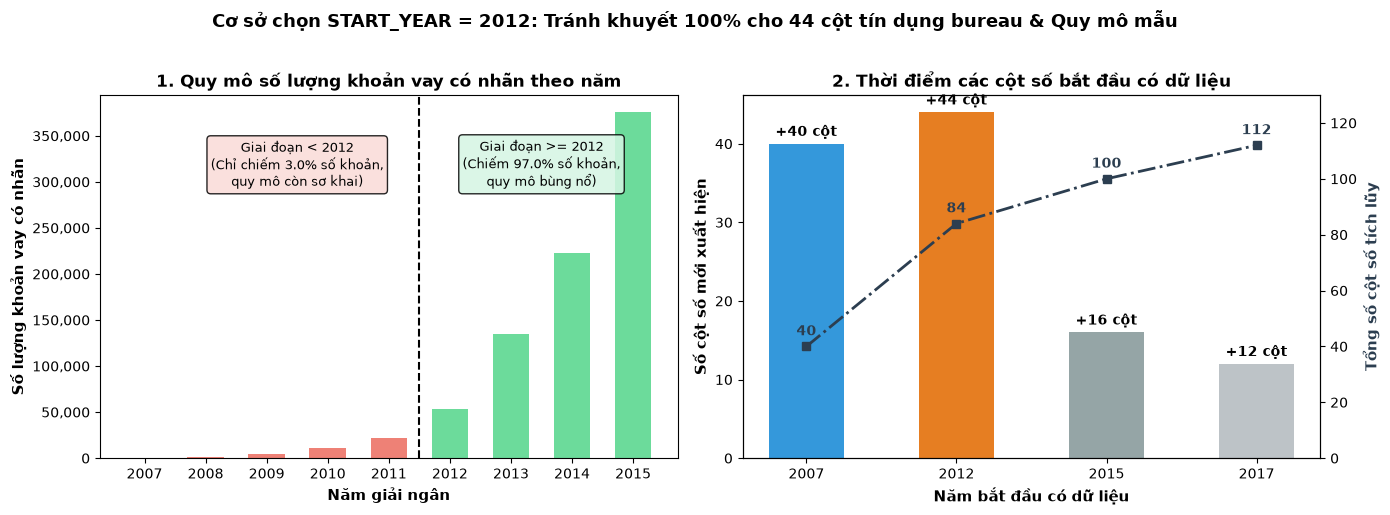
\includegraphics[width=\textwidth]{Images/start_year.png}
\caption{Left: number of labelled loans per issue year up to 2015, with the pre-2012 share. Right: number of numeric columns that first have data in each year, with the cumulative count.}
\label{fig:startyear}
\end{figure}

\paragraph{Maturity rule and filters.} Table~\ref{tab:maturity} verifies the matured-loan rule: 99.6\% of the 676,459 matured loans have a final label against 42.4\% of the 1,584,242 unmatured ones. The default rate in the matured group is 14.8\% (against 25.1\% for the unmatured loans that happen to be labelled), and only 8.2\% of matured loans are 60-month, which is why Section~\ref{sec:filters} restricts to 36-month loans. Table~\ref{tab:funnel} shows the funnel: 589,488 loans, 26.1\% of the file, remain; the 36-month filter removes 7.0\% of the loans left after the maturity rule.

\begin{table}[H]
\centering
\caption{Check of the matured-loan rule.}
\label{tab:maturity}
\begin{tabular}{lrrrr}
\toprule
\textbf{Group} & \textbf{Loans} & \textbf{Labelled share} & \textbf{Default rate} & \textbf{60-month share} \\
\midrule
Unmatured & 1,584,242 & 0.424 & 0.251 & 0.376 \\
Matured & 676,459 & 0.996 & 0.148 & 0.082 \\
\bottomrule
\end{tabular}
\end{table}

\begin{table}[H]
\centering
\caption{Filtering funnel.}
\label{tab:funnel}
\begin{tabular}{lrrr}
\toprule
\textbf{Step} & \textbf{Rows} & \textbf{Retained (\%)} & \textbf{Step reduction (\%)} \\
\midrule
Raw data & 2,260,701 & 100.00 & 0.00 \\
Labelled (Fully Paid / Charged Off) & 1,345,310 & 59.51 & 40.49 \\
\quad and issued from 2012 & 1,305,524 & 57.75 & 2.96 \\
\quad and matured & 633,767 & 28.03 & 51.46 \\
\quad and 36-month term & 589,488 & 26.08 & 6.99 \\
\bottomrule
\end{tabular}
\end{table}

\paragraph{The split.} Table~\ref{tab:split} gives the three sets. The cut dates are 2015-06-01 and 2015-10-01. The training set holds 69.2\% of the loans, spans 41 months and has a 13.7\% default rate; validation and test are 15.7\% and 15.0\% with default rates 14.7\% and 14.8\%. All three sets contain only 36-month loans, so the term mix is identical. The manifest hash of the sorted training ids is \texttt{8ce37fef31257778922ffe920c32511c}. Figure~\ref{fig:timesplit} shows loan counts and default rate by issue month with the cut lines, and Figure~\ref{fig:target} the label balance and the default rate per set. The default-rate gap between the largest and smallest set is 0.011, i.e.\ a mild but real drift that the models will face.

\begin{table}[H]
\centering
\caption{Train, validation and test sets.}
\label{tab:split}
\begin{tabular}{lrrccc}
\toprule
\textbf{Set} & \textbf{Loans} & \textbf{\% of total} & \textbf{From} & \textbf{To} & \textbf{Default rate} \\
\midrule
Train & 408,188 & 69.24 & 2012-01 & 2015-05 & 0.137 \\
Validation & 92,631 & 15.71 & 2015-06 & 2015-09 & 0.147 \\
Test & 88,669 & 15.04 & 2015-10 & 2015-12 & 0.148 \\
\bottomrule
\end{tabular}
\end{table}

\begin{figure}[H]
\centering
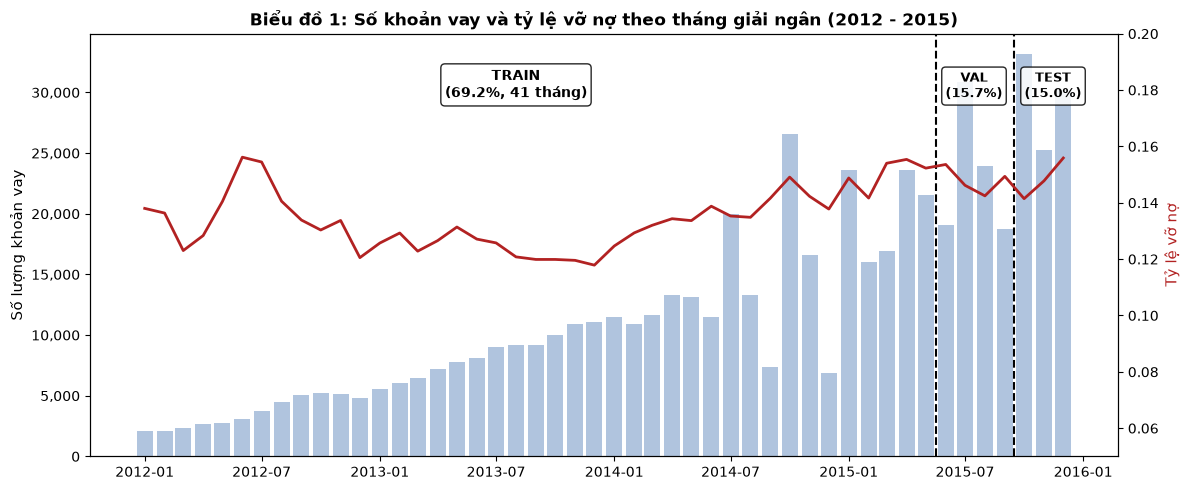
\includegraphics[width=0.95\textwidth]{Images/time_split.png}
\caption{Number of loans (bars) and default rate (line) by issue month, 2012--2015, with the two cut dates separating train, validation and test.}
\label{fig:timesplit}
\end{figure}

\begin{figure}[H]
\centering
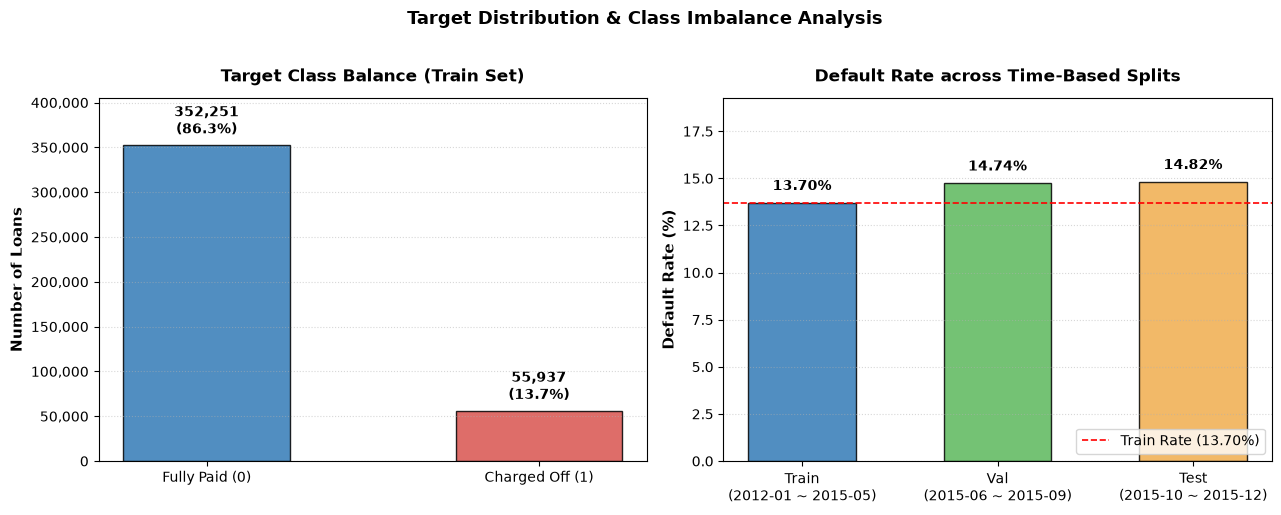
\includegraphics[width=0.95\textwidth]{Images/target_balance.png}
\caption{Left: label balance in the training set. Right: default rate in each time-based set.}
\label{fig:target}
\end{figure}

\paragraph{Label maturity at the end of the window.} For 36-month loans issued in 2015 the final-label rate is 100.0\% in every month from January to October, 99.9\% in November and 99.7\% in December (99.68\%). The test period therefore has about 0.3\% of its December loans still without a final outcome; this is a known, small limitation (Section~\ref{sec:limits}).

\paragraph{Missing values.} In the training set, 53 columns have no missing values, 66 are partially missing and 32 are entirely empty (Figure~\ref{fig:missing}). Seventeen of the 32 empty columns do have values in validation or test because Lending Club began recording them after the training period; a model cannot learn from them, so they are excluded. The \code{desc} column shows the largest train--test shift in missing share (18.4 percentage points).

\begin{figure}[H]
\centering
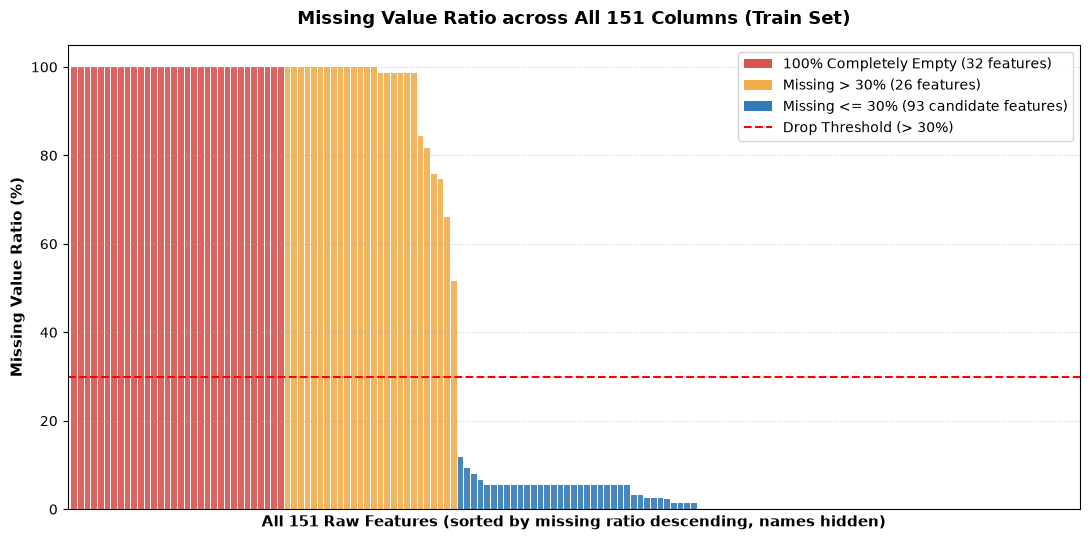
\includegraphics[width=0.85\textwidth]{Images/missing_values.png}
\caption{Share of missing values for each of the 151 raw columns in the training set (sorted; names hidden). The dashed line marks the 30\% drop threshold.}
\label{fig:missing}
\end{figure}

\subsection{Evidence for the leakage controls and the column groups}
\label{sec:res-leak}

Table~\ref{tab:leak} lists the ten suspect (post-origination or uncertain-timing) columns with the highest single-column training AUC. Of the 42 suspect columns, 10 exceed the best application-time column, which is \code{sub\_grade} with AUC 0.6565 (73 application-time columns were scored). The top suspects reach 0.9074 (\code{last\_fico\_range\_low} and \code{last\_fico\_range\_high}), 0.9054 (\code{recoveries}) and 0.8677 (\code{collection\_recovery\_fee}). These columns record what happened \emph{after} the loan, so a model that used them would appear far better than any application-time model; the check supports the whitelist rule empirically. Note that the AUC of text columns with few values is computed in-sample (Section~\ref{sec:leakage}), which may overstate the single-column strength of \code{sub\_grade} (it is scored on the same data from which its group means are taken), so 0.6565 should be read with that caveat.

\begin{table}[H]
\centering
\caption{Suspect columns with the highest single-column ROC-AUC on the training set (best application-time column: \code{sub\_grade}, 0.6565).}
\label{tab:leak}
\small
\begin{tabular}{lrl}
\toprule
\textbf{Column} & \textbf{AUC} & \textbf{Meaning} \\
\midrule
last\_fico\_range\_low & 0.9074 & Lower FICO bound at the latest credit pull \\
last\_fico\_range\_high & 0.9074 & Upper FICO bound at the latest credit pull \\
recoveries & 0.9054 & Amount recovered after charge-off \\
collection\_recovery\_fee & 0.8677 & Collection fee after charge-off \\
last\_credit\_pull\_d & 0.8355 & Month of the latest credit pull \\
total\_rec\_prncp & 0.8280 & Principal received to date \\
last\_pymnt\_amnt & 0.7673 & Amount of the latest payment \\
total\_pymnt & 0.7554 & Total payments received to date \\
total\_pymnt\_inv & 0.7554 & Total payments received (investor portion) \\
last\_pymnt\_d & 0.6577 & Month of the latest payment \\
\bottomrule
\end{tabular}
\end{table}

Table~\ref{tab:groups} and Figure~\ref{fig:groups} show the outcome of the rule groups: from 151 columns, 57 candidates (38\%) remain. The 42 post-origination or uncertain columns and the 32 columns empty in training are the largest removed groups. All 16 joint-application columns are empty in the training set (every training loan is an \code{Individual} application; the test set contains 0.3\% \code{Joint App}), so they fall under the ``empty'' rule. A code assertion confirms that no column of the leakage group is among the 57 candidates.

\begin{table}[H]
\centering
\caption{Number of the 151 raw columns in each rule group.}
\label{tab:groups}
\begin{tabular}{lr}
\toprule
\textbf{Group} & \textbf{Columns} \\
\midrule
Kept as candidates & 57 \\
Post-origination / uncertain timing & 42 \\
Empty in train & 32 \\
(Quasi-)constant & 7 \\
Missing $>30\%$ in train & 5 \\
High-cardinality text & 4 \\
Identifier & 2 \\
Label / auxiliary & 2 \\
\midrule
\textbf{Total} & \textbf{151} \\
\bottomrule
\end{tabular}
\end{table}

\begin{figure}[H]
\centering
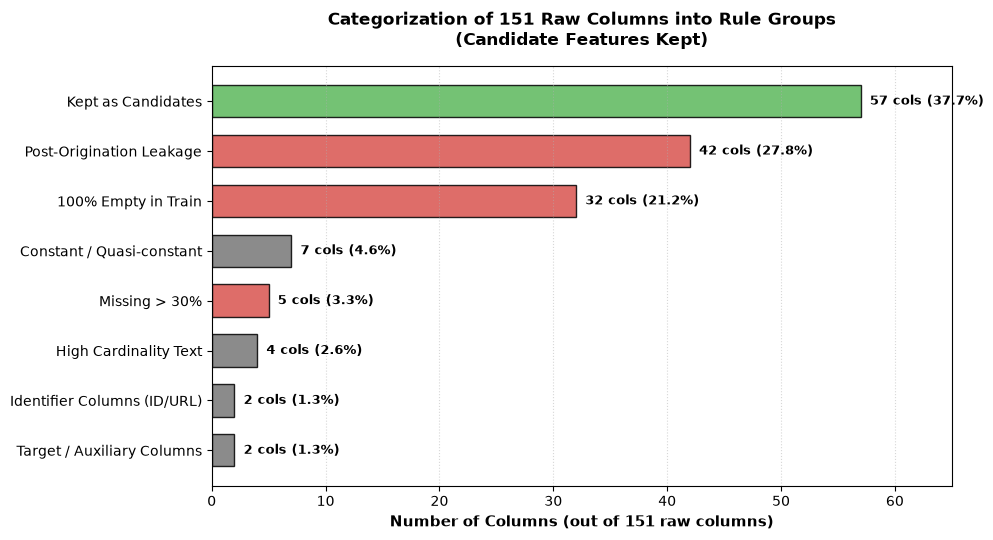
\includegraphics[width=0.85\textwidth]{Images/column_groups.png}
\caption{Categorisation of the 151 raw columns into rule groups; green marks the 57 candidate columns.}
\label{fig:groups}
\end{figure}

Because the five columns in the ``missing $>30\%$'' group are the \code{mths\_since\_...} variables (months since last delinquency, public record, major derogatory item, bank-card delinquency and revolving delinquency), their information is lost; it is a deliberate simplification, and an indicator-based treatment is listed as future work. Of the remaining candidates, 26 columns are 5--30\% missing in the training set; all of them first appear in the data in 2012 and are median-imputed.

\subsection{Cleaning checks, EDA and feature selection}
\label{sec:res-eda}

\paragraph{Logic checks.} Table~\ref{tab:logic} counts violations of the business rules before and after cleaning. The rules \code{annual\_inc}$\le 0$, \code{dti}$<0$ and \code{dti}$>100$ have no violations in training but do occur in validation/test (2 and 5 rows in test); the rules were set from the meaning of the columns, not from validation or test. After cleaning, the corrected rules are at zero in all three sets; \code{revol\_util}$>100$ (1,321 / 421 / 461 rows) is kept because it is possible, only the extreme values are capped at 102.4. There are no duplicate or cross-set loan ids.

\begin{table}[H]
\centering
\caption{Rows violating each logic rule before cleaning (after cleaning, only \code{revol\_util}$>100$ remains because it is a valid case).}
\label{tab:logic}
\small
\begin{tabular}{lrrr}
\toprule
\textbf{Rule} & \textbf{Train} & \textbf{Validation} & \textbf{Test} \\
\midrule
annual\_inc $\le 0$ & 0 & 0 & 2 \\
dti $<0$ & 0 & 0 & 0 \\
dti $>100$ & 0 & 0 & 5 \\
revol\_util $>100$ & 1,321 & 421 & 461 \\
fico\_range\_low $>$ fico\_range\_high & 0 & 0 & 0 \\
first credit line after issue date & 0 & 0 & 0 \\
loan\_amnt $\le 0$ & 0 & 0 & 0 \\
\bottomrule
\end{tabular}
\end{table}

\paragraph{Default rate versus key variables.} Figure~\ref{fig:purpose} shows the default rate by loan purpose in the training set: it is highest for \code{small\_business} (22.4\%) and lowest for \code{car} (11.4\%) and \code{credit\_card} (11.5\%); the \code{educational} bar is 0.0\% (the notebook does not print the number of such loans, so we do not interpret it). Figure~\ref{fig:subgrade} shows that the default rate rises monotonically with sub-grade, from 2.7\% for A1 to 36.4\% for G5: the platform's grade is a strong, ordered risk signal. Figure~\ref{fig:intrate} shows that the interest rate is tiered by grade, which is why \code{int\_rate} would duplicate the incumbent score and is dropped.

\begin{figure}[H]
\centering
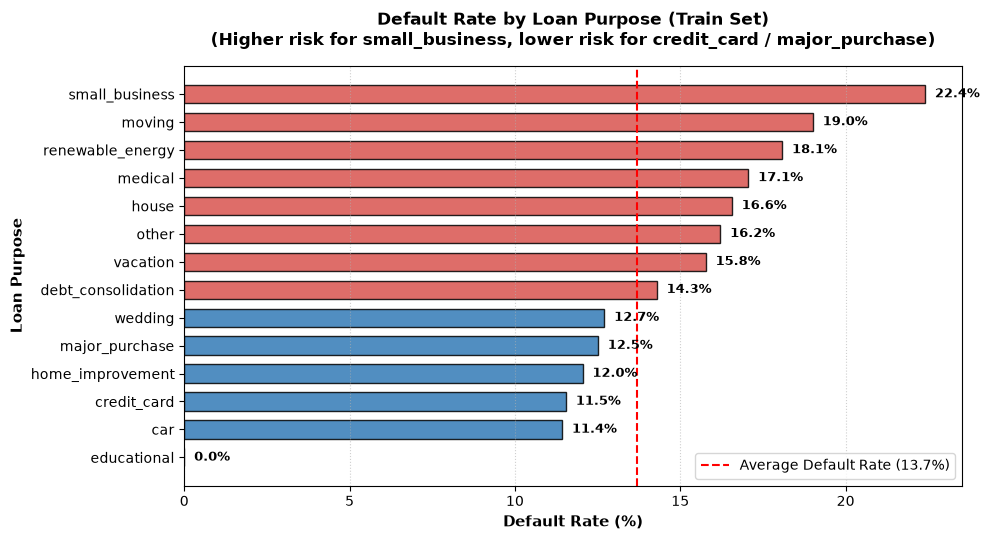
\includegraphics[width=0.85\textwidth]{Images/purpose.png}
\caption{Default rate by loan purpose in the training set (dashed line: overall 13.7\%).}
\label{fig:purpose}
\end{figure}

\begin{figure}[H]
\centering
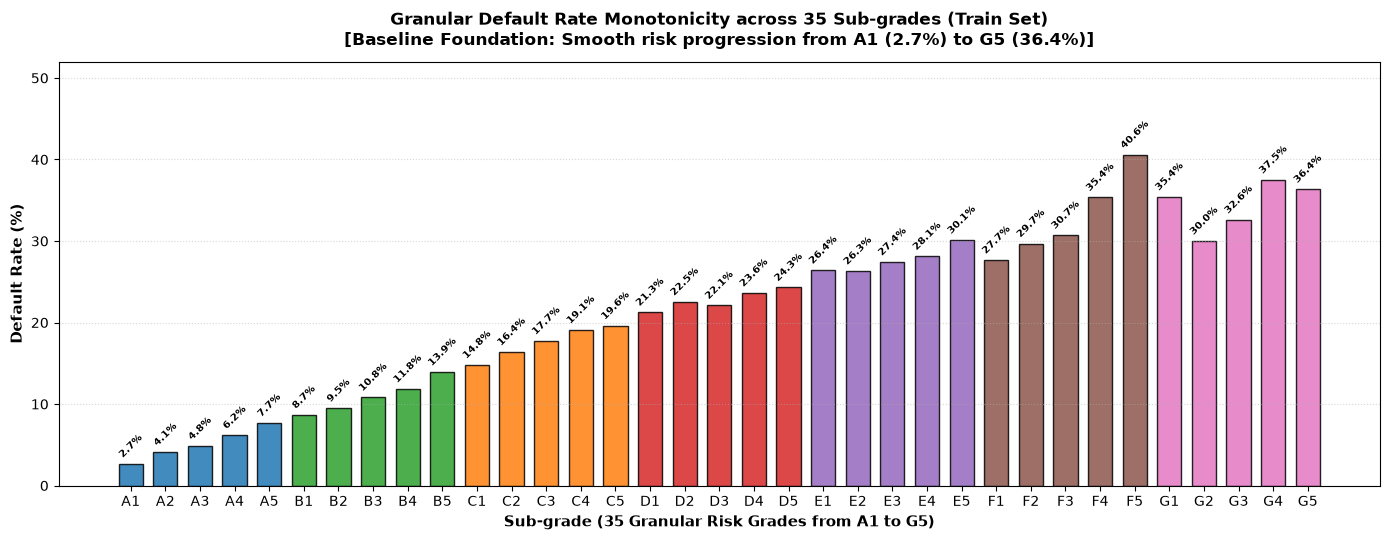
\includegraphics[width=\textwidth]{Images/subgrade_rate.png}
\caption{Default rate by sub-grade (A1--G5) in the training set.}
\label{fig:subgrade}
\end{figure}

\begin{figure}[H]
\centering
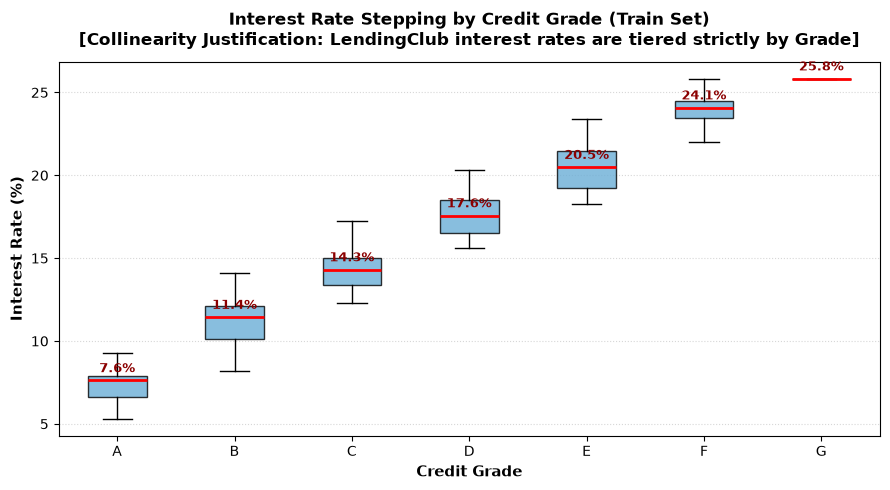
\includegraphics[width=0.75\textwidth]{Images/interest_by_grade.png}
\caption{Distribution of the interest rate by grade in the training set; rates step up with the grade.}
\label{fig:intrate}
\end{figure}

\paragraph{Behaviour of the main numeric features.} Figure~\ref{fig:decile} gives the default rate within each decile of six features (training set, overall rate 13.7\%). Risk falls steadily as \code{fico\_avg} rises (18.6\% in the lowest decile, median FICO 662, to 5.7\% in the highest, median 762) and as \code{annual\_inc} rises (20.0\% to 9.1\%), and rises with \code{dti} (10.5\% to 19.1\%), \code{revol\_util} (10.3\% to 16.2\%) and \code{loan\_to\_income} (10.7\% to 18.5\%). \code{loan\_amnt} is \emph{not} monotone: its default rate peaks at 15.7\% in decile 4 and ends at 12.4\% in decile 10. A linear term in the logistic model therefore cannot capture the loan-amount pattern, which is one reason non-linear models are worth testing. Figure~\ref{fig:newfeat} compares the engineered \code{fico\_avg} and \code{loan\_to\_income} between repaid and defaulted loans: the median FICO is lower and the median loan-to-income higher for defaulted loans.

\begin{figure}[H]
\centering
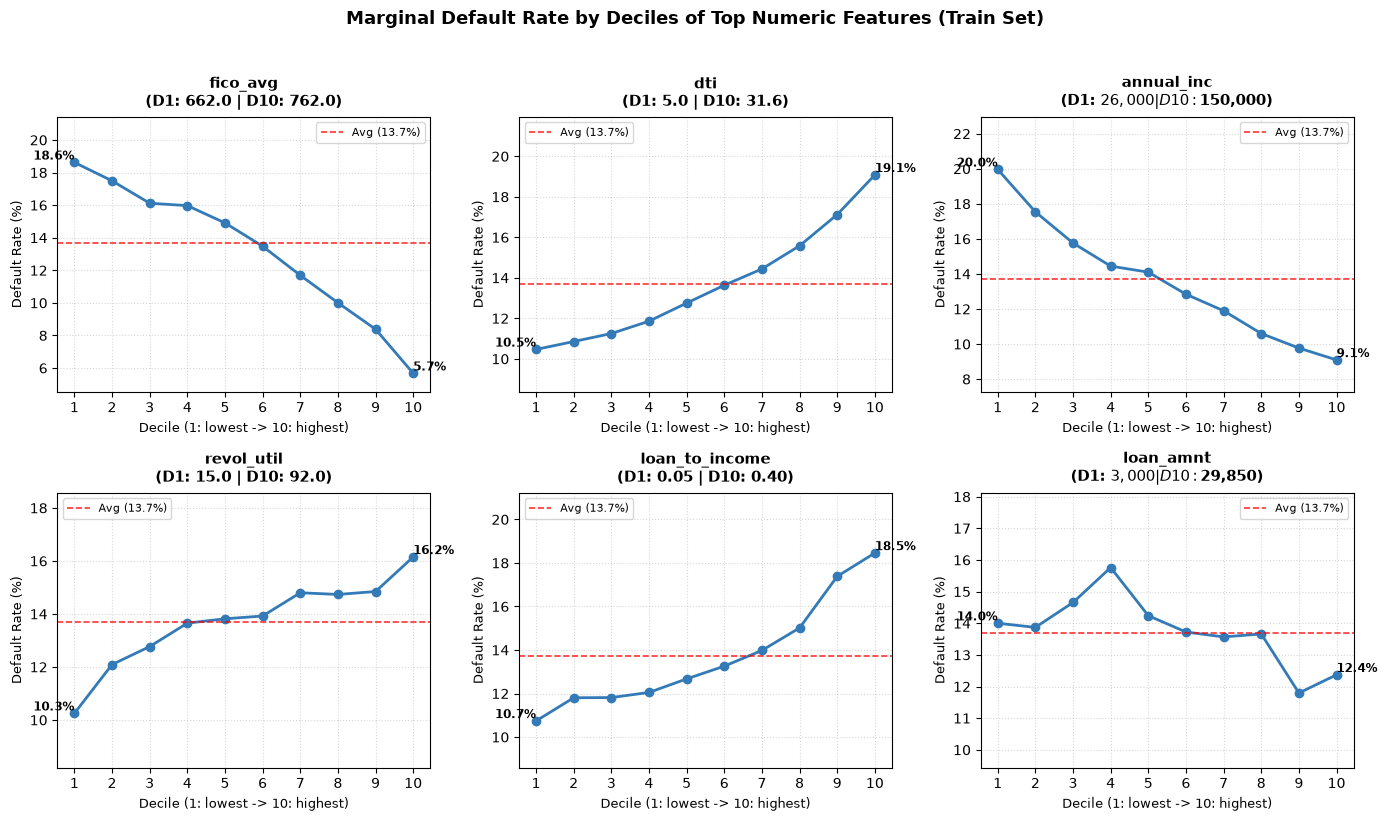
\includegraphics[width=\textwidth]{Images/decile.png}
\caption{Default rate by decile of six numeric features in the training set (dashed line: overall default rate). Titles give the median value of the first and last decile; matplotlib renders the two dollar signs in some titles as mathematical text.}
\label{fig:decile}
\end{figure}

\begin{figure}[H]
\centering
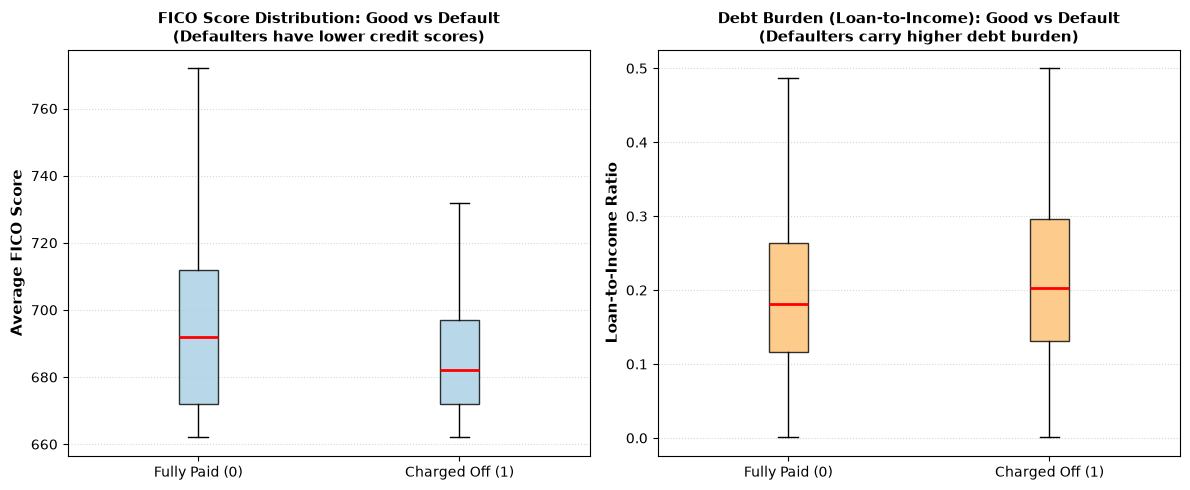
\includegraphics[width=0.85\textwidth]{Images/new_features.png}
\caption{Box plots (outliers hidden) of \code{fico\_avg} and \code{loan\_to\_income} for repaid and defaulted loans in the training set.}
\label{fig:newfeat}
\end{figure}

\paragraph{Single-feature strength and collinearity.} Figure~\ref{fig:uniauc} ranks the numeric candidates by single-column AUC on the training set: \code{int\_rate} (0.650) is the strongest, followed by \code{fico\_avg} (0.598) and \code{log\_annual\_inc} (0.580); \code{int\_rate} is shown only for comparison, as it was later dropped. The best purely numeric application-time feature thus has an AUC of about 0.60, compared with 0.6565 for \code{sub\_grade} alone, which already indicates that a model must combine many weak signals to beat the incumbent.

Five numeric pairs have $|r|\ge0.90$ in the training set (Table~\ref{tab:corr}; Figure~\ref{fig:corr} for eight key features); in each pair the column with the lower single-column AUC is dropped (\code{open\_acc}, \code{installment}, \code{num\_rev\_tl\_bal\_gt\_0}, \code{tot\_cur\_bal}, \code{credit\_history\_years}). Together with \code{int\_rate} and the constant \code{term\_months}, this reduces 52 numeric candidates to 45; with the five categorical columns (\code{sub\_grade}, \code{home\_ownership}, \code{verification\_status}, \code{purpose}, \code{addr\_state}) the model has 50 input features and 153 columns after one-hot encoding.

\begin{figure}[H]
\centering
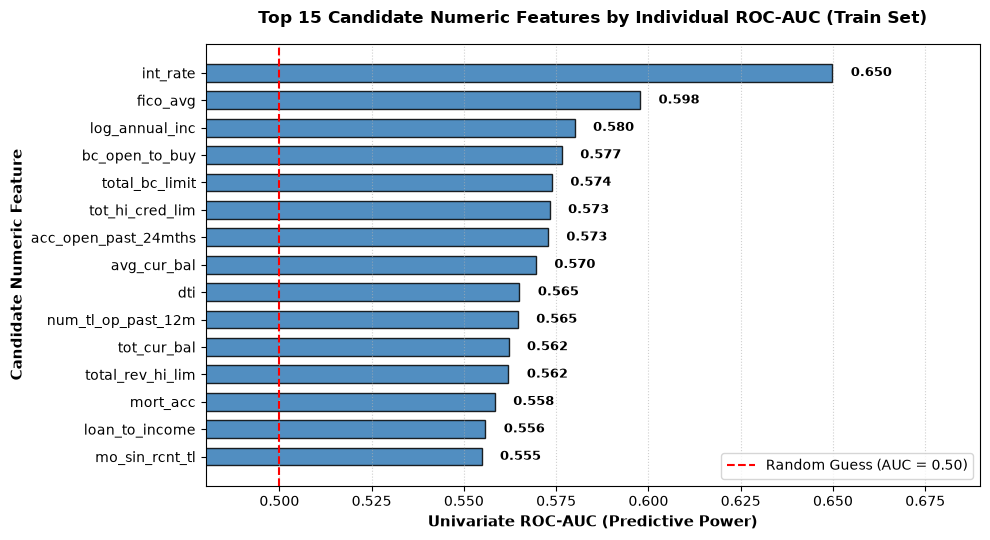
\includegraphics[width=0.85\textwidth]{Images/univariate_auc.png}
\caption{Top 15 numeric candidates by single-column ROC-AUC in the training set.}
\label{fig:uniauc}
\end{figure}

\begin{table}[H]
\centering
\caption{Numeric column pairs with $|r|\ge0.90$ in the training set and the column dropped.}
\label{tab:corr}
\small
\begin{tabular}{llcrrl}
\toprule
\textbf{Column A} & \textbf{Column B} & \textbf{$r$} & \textbf{AUC A} & \textbf{AUC B} & \textbf{Dropped} \\
\midrule
open\_acc & num\_sats & 0.9987 & 0.5065 & 0.5071 & open\_acc \\
loan\_amnt & installment & 0.9941 & 0.5179 & 0.5044 & installment \\
num\_actv\_rev\_tl & num\_rev\_tl\_bal\_gt\_0 & 0.9903 & 0.5398 & 0.5395 & num\_rev\_tl\_bal\_gt\_0 \\
tot\_cur\_bal & tot\_hi\_cred\_lim & 0.9744 & 0.5621 & 0.5732 & tot\_cur\_bal \\
mo\_sin\_old\_rev\_tl\_op & credit\_history\_years & 0.9245 & 0.5492 & 0.5400 & credit\_history\_years \\
\bottomrule
\end{tabular}
\end{table}

\begin{figure}[H]
\centering
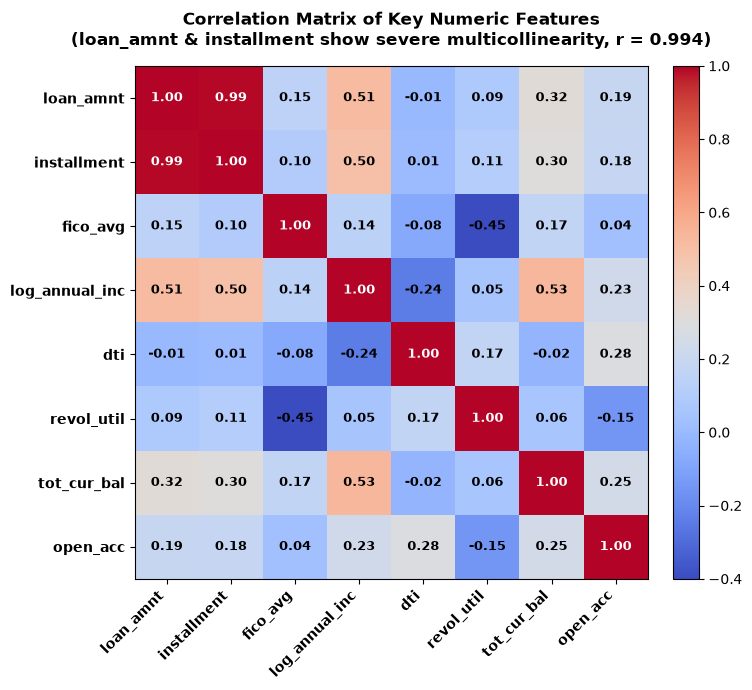
\includegraphics[width=0.7\textwidth]{Images/corr.png}
\caption{Pearson correlation matrix of eight key numeric features in the training set; \code{loan\_amnt} and \code{installment} have $r=0.994$.}
\label{fig:corr}
\end{figure}

\subsection{Evidence for the preprocessing choices}
\label{sec:res-prep}

\paragraph{Median versus mean imputation.} Of the 45 numeric features, 31 have missing values in the training set. Of these, 28 are right-skewed (skewness $>0$) and 25 strongly so (skewness $>1$); the most extreme are \code{tot\_coll\_amt} (skewness 606.4) and \code{total\_rev\_hi\_lim} (97.2). For several balance and limit columns the mean is far above the median (for example \code{avg\_cur\_bal}: mean 12,502.7 versus median 6,228.0, +100.7\%; \code{tot\_hi\_cred\_lim}: 156,218.6 versus 91,316.0, +71.1\%). Figure~\ref{fig:skew} summarises the skewness and mean/median ratio for the most skewed columns, and Figure~\ref{fig:impute} shows that filling with the mean creates an artificial spike away from the bulk of the distribution (\code{total\_rev\_hi\_lim}), whereas the median fill sits within it. We therefore use median imputation.

\begin{figure}[H]
\centering
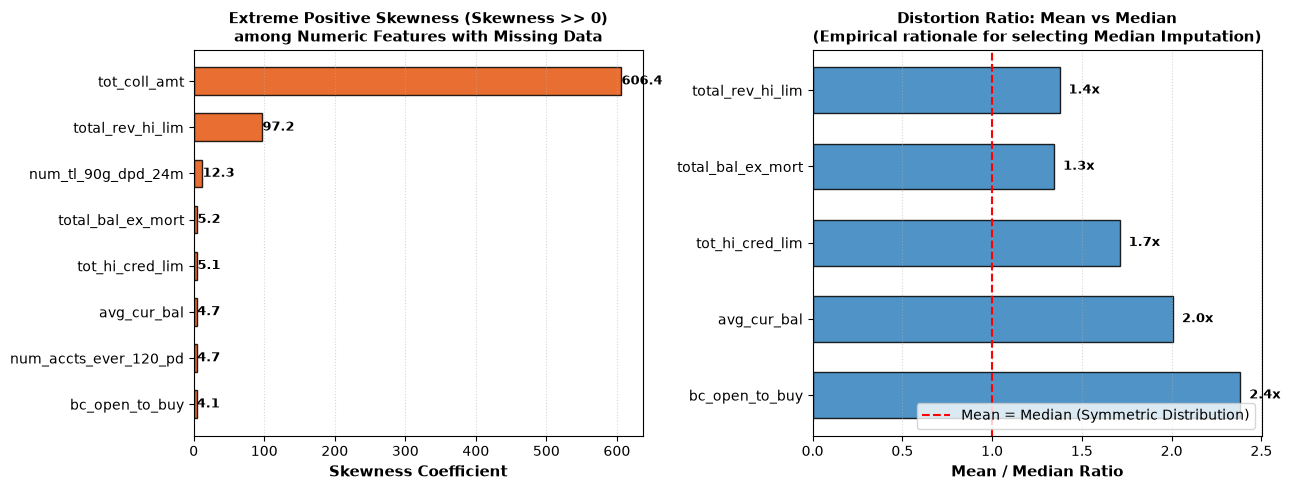
\includegraphics[width=\textwidth]{Images/skew.png}
\caption{Left: skewness of the most skewed numeric features with missing data. Right: mean-to-median ratio for the same features.}
\label{fig:skew}
\end{figure}

\begin{figure}[H]
\centering
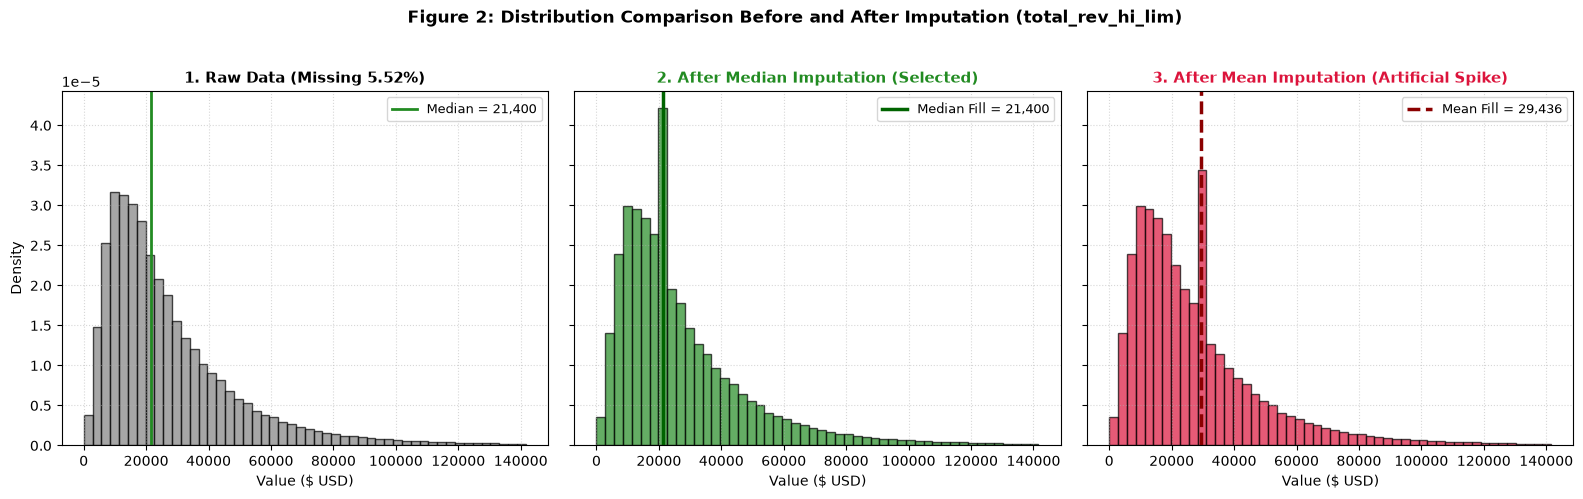
\includegraphics[width=\textwidth]{Images/imputation.png}
\caption{Distribution of \code{total\_rev\_hi\_lim} (below the 99th percentile): raw data, after median imputation and after mean imputation.}
\label{fig:impute}
\end{figure}

\paragraph{Standardisation.} On a 10,000-loan sample of the training set, the raw means range from 0.34 (\code{delinq\_2yrs}) to 127,162 (\code{tot\_cur\_bal}), a ratio above $10^{5}$ (Figure~\ref{fig:scale-before}). After \code{StandardScaler} every feature has mean about 0 (maximum $|\mu|=5.07\times10^{-16}$) and standard deviation 1.0001 (Figure~\ref{fig:scale-after}). This matters for Equation~\eqref{eq:lr}, because the L2 penalty would otherwise penalise features unequally depending on their units, and it makes coefficient sizes comparable.

\begin{figure}[H]
\centering
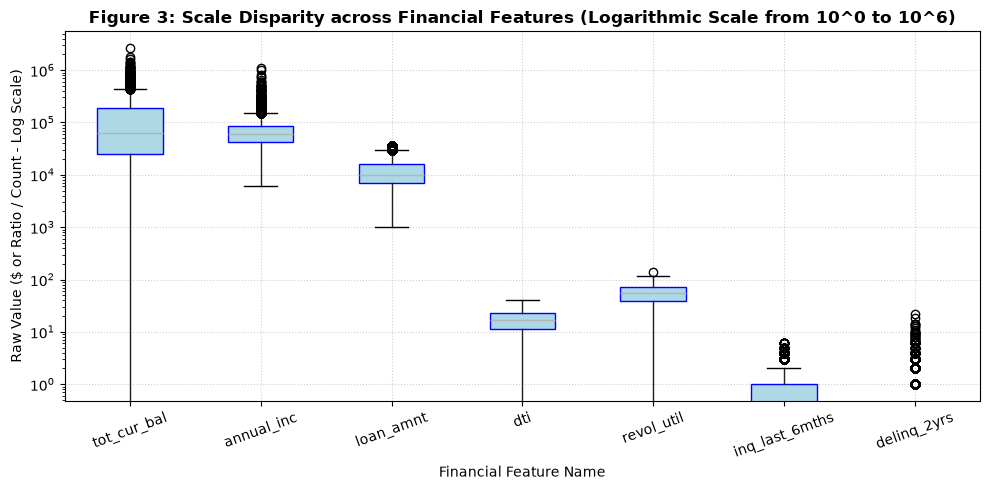
\includegraphics[width=0.85\textwidth]{Images/scale_before.png}
\caption{Raw scale of seven financial features (logarithmic axis) in a sample of 10,000 training loans.}
\label{fig:scale-before}
\end{figure}

\begin{figure}[H]
\centering
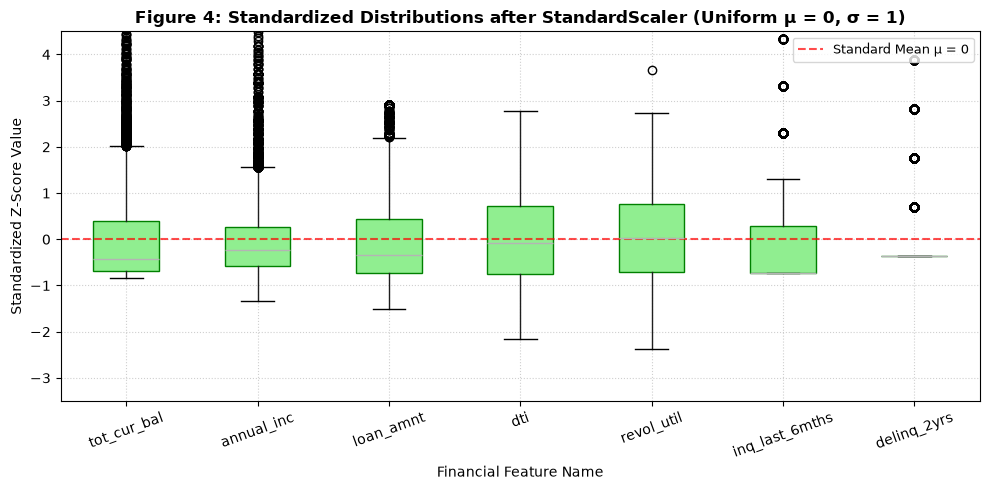
\includegraphics[width=0.85\textwidth]{Images/scale_after.png}
\caption{The same features after standardisation.}
\label{fig:scale-after}
\end{figure}

\paragraph{No leakage through the pipeline.} The pipeline output has 153 columns for train, validation and test and no remaining missing values. After scaling, the training means are zero (maximum absolute mean $6.39\times10^{-16}$) whereas the validation means are not (maximum absolute mean 0.162), as expected when validation is transformed with training statistics. A second fit on the training set reproduces the same validation matrix (\code{allclose} is true), so the preprocessing is deterministic.

\subsection{Model comparison}
\label{sec:res-models}

\subsubsection{Hyperparameter tuning}

Table~\ref{tab:tune} summarises the time-ordered cross-validated ROC-AUC (mean over three folds, inside the training set) for the selected configurations. For logistic regression the CV AUC is 0.6855 at $C=1$ and 0.6854 at $C=10$, 0.6853 at $C=0.1$, 0.6839 at $C=0.01$ and 0.6782 at $C=0.001$: the score is flat for $C\ge0.1$, and the largest penalty is clearly worse. For the decision tree the best depth is 7 (CV AUC 0.6355), with shallower and deeper trees lower (depth 3: 0.6139; depth 10: 0.6278). The best random forest has 150 trees, depth 10 and minimum leaf 50 (0.6741); the best gradient-boosting model has 150 iterations, depth 10 and learning rate 0.05 (0.6852). In the random-forest grid the depth-10 settings occupy the top nine places (CV AUC 0.6720--0.6741), and the first depth-8 configuration is 0.6710; in the boosting grid, the ten best configurations lie within 0.0018 of each other (CV AUC 0.6852 to 0.6834).

\begin{table}[H]
\centering
\caption{Selected hyperparameters and cross-validated ROC-AUC (\code{TimeSeriesSplit(3)} inside the training set).}
\label{tab:tune}
\small
\begin{tabular}{llr}
\toprule
\textbf{Model} & \textbf{Selected hyperparameters} & \textbf{CV AUC} \\
\midrule
Logistic regression & $C=1.0$ & 0.6855 \\
Decision tree & \code{max\_depth}=7, \code{min\_samples\_leaf}=50 & 0.6355 \\
Random forest & 150 trees, \code{max\_depth}=10, \code{min\_samples\_leaf}=50 & 0.6741 \\
HistGradientBoosting & \code{max\_iter}=150, \code{max\_depth}=10, \code{learning\_rate}=0.05 & 0.6852 \\
\bottomrule
\end{tabular}
\end{table}

The random-forest and boosting selections sit on the edge of their grids (trees 150, depth 10; boosting iterations 150, depth 10, learning rate 0.05), so a wider search could find better settings; Section~\ref{sec:limits} discusses this.

\subsubsection{Validation performance and overfitting check}

Table~\ref{tab:valperf} gives the validation results with the train--validation AUC gap, and Figure~\ref{fig:models} plots the ROC curves and the three metrics. The \code{sub\_grade} baseline reaches validation AUC 0.6815 (Gini 36.31\%, KS 27.02\%). Logistic regression (0.7040) and HistGradientBoosting (0.7054) are the best two models; their Gini values are 40.79\% and 41.07\% and their KS values 29.94\% and 30.02\%. The random forest (0.6876) is above the baseline but below both; the decision tree (0.6536) is below the baseline.

\begin{table}[H]
\centering
\caption{Model comparison on the validation set (92,631 loans) and train--validation AUC gap.}
\label{tab:valperf}
\small
\begin{tabular}{lccccc}
\toprule
\textbf{Model} & \textbf{AUC train} & \textbf{AUC val} & \textbf{Gap (train--val)} & \textbf{Gini val} & \textbf{KS val} \\
\midrule
Baseline \code{sub\_grade} & 0.6565 & 0.6815 & $-0.0250$ & 36.31\% & 27.02\% \\
Logistic L2 ($C=1$) & 0.6873 & 0.7040 & $-0.0167$ & 40.79\% & 29.94\% \\
Decision tree (depth 7) & 0.6541 & 0.6536 & $+0.0006$ & 30.71\% & 22.25\% \\
Random forest (150, depth 10) & 0.7060 & 0.6876 & $+0.0184$ & 37.52\% & 27.21\% \\
HistGradientBoosting & 0.7096 & 0.7054 & $+0.0042$ & 41.07\% & 30.02\% \\
\bottomrule
\end{tabular}
\end{table}

\begin{figure}[H]
\centering
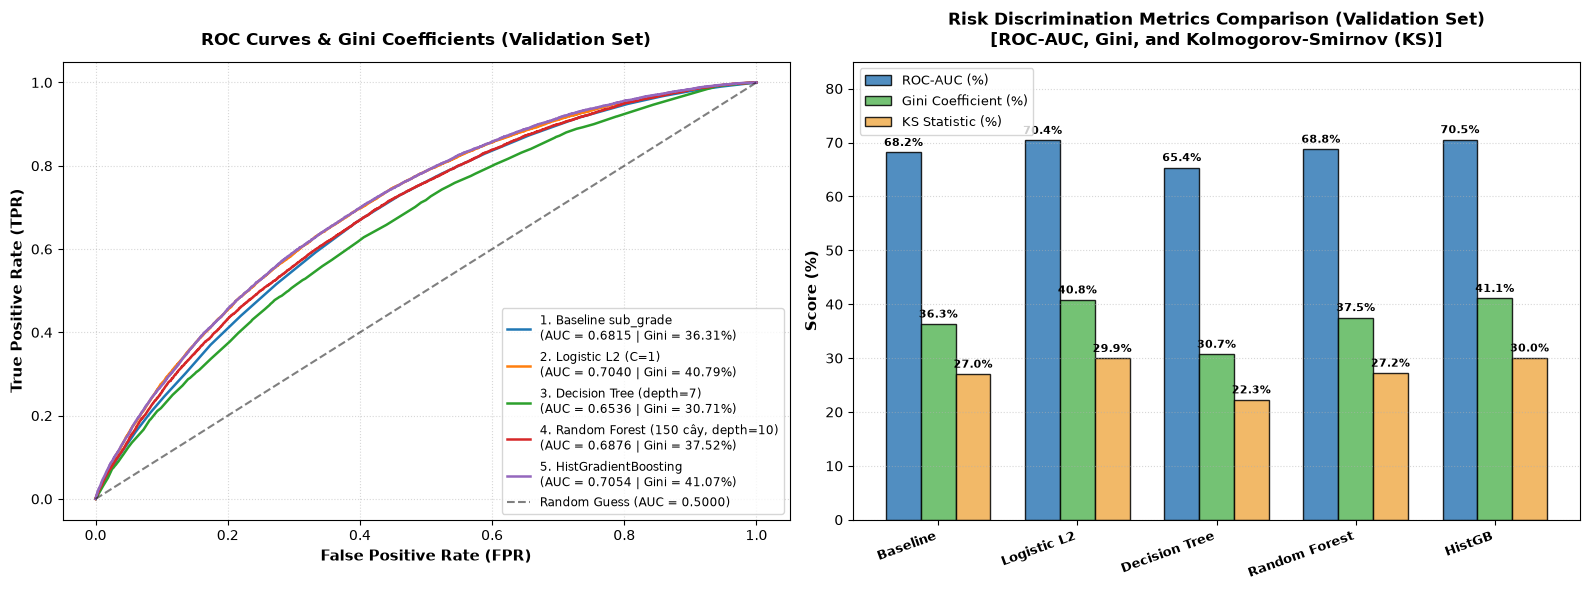
\includegraphics[width=\textwidth]{Images/model_comparison.png}
\caption{Validation set. Left: ROC curves with AUC and Gini of the five models. Right: ROC-AUC, Gini and KS of each model.}
\label{fig:models}
\end{figure}

The overfitting check gives a mixed picture. The random forest has the largest positive gap ($+0.0184$): it fits the training period noticeably better than the later validation period. HistGradientBoosting has a gap of $+0.0042$ and the decision tree $+0.0006$. For the baseline ($-0.0250$) and logistic regression ($-0.0167$) the \emph{validation} AUC is higher than the training AUC. This means the validation months were easier to rank for these two models, not that they generalise better in any deeper sense; we did not isolate the cause (a change over time in how sharply sub-grade separates defaults would be one candidate), so we only report the observation.

Figure~\ref{fig:ks} shows the cumulative separation curves of defaulters and non-defaulters ordered by score for the baseline and logistic regression, from which the KS values in Table~\ref{tab:valperf} are read as the maximum vertical gap.

\begin{figure}[H]
\centering
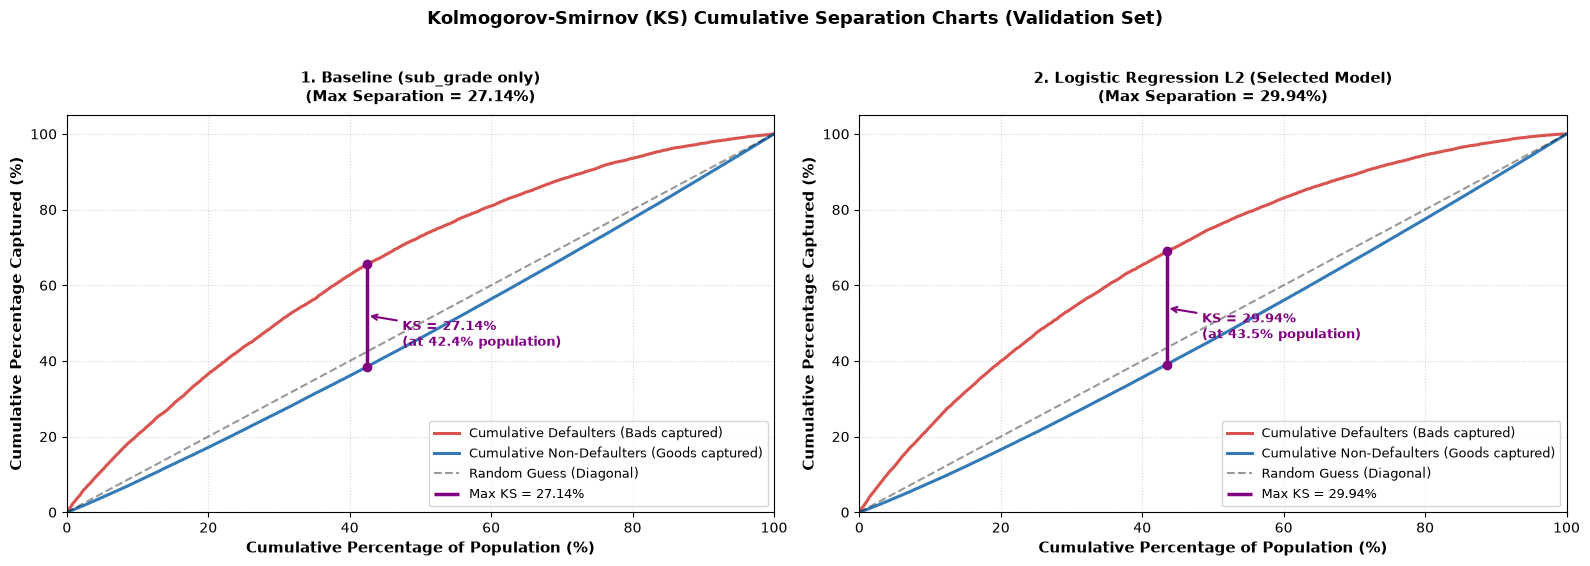
\includegraphics[width=\textwidth]{Images/ks_curve.png}
\caption{Cumulative separation (KS) charts on the validation set for the baseline (left) and logistic regression (right).}
\label{fig:ks}
\end{figure}

\subsubsection{Bootstrap confidence intervals}

Table~\ref{tab:boot} gives the paired-bootstrap results on the validation set (1,000 resamples). Logistic regression improves the AUC over the baseline by $+0.0225$ (95\% CI $[+0.0196,+0.0253]$), HistGradientBoosting by $+0.0238$ ($[+0.0206,+0.0270]$) and the random forest by $+0.0061$ ($[+0.0024,+0.0102]$); all three intervals exclude zero. The decision tree is below the baseline ($-0.0280$, $[-0.0329,-0.0233]$). Comparing the two best models directly gives HistGB minus logistic regression $=[-0.0002,+0.0031]$, an interval that contains zero: on this validation set we cannot distinguish them, even though the point estimate favours boosting by about $+0.0014$.

\begin{table}[H]
\centering
\caption{Paired-bootstrap difference in validation AUC against the \code{sub\_grade} baseline ($B=1{,}000$).}
\label{tab:boot}
\small
\begin{tabular}{lcc}
\toprule
\textbf{Model} & \textbf{Mean $\Delta$AUC} & \textbf{95\% CI} \\
\midrule
Logistic L2 ($C=1$) & $+0.0225$ & $[+0.0196,+0.0253]$ \\
Decision tree (depth 7) & $-0.0280$ & $[-0.0329,-0.0233]$ \\
Random forest (150, depth 10) & $+0.0061$ & $[+0.0024,+0.0102]$ \\
HistGradientBoosting & $+0.0238$ & $[+0.0206,+0.0270]$ \\
\midrule
HistGB $-$ Logistic L2 & --- & $[-0.0002,+0.0031]$ \\
\bottomrule
\end{tabular}
\end{table}

\subsubsection{Final evaluation on the test set}

The test set (88,669 loans issued October--December 2015) was evaluated once for the baseline, logistic regression and HistGradientBoosting (Table~\ref{tab:test}). The baseline reaches AUC 0.6818 (Gini 36.36\%, KS 26.45\%); logistic regression 0.7039 (Gini 40.79\%, KS 29.87\%), i.e.\ $+0.0221$; HistGradientBoosting 0.7055 (Gini 41.10\%, KS 29.97\%), i.e.\ $+0.0237$. The test values are almost identical to the validation values (baseline 0.6815 versus 0.6818; logistic regression 0.7040 versus 0.7039; HistGB 0.7054 versus 0.7055), so the ranking of the three models and the size of the gain are stable from validation to test. In Gini terms the models add about 4.4 (logistic) and 4.7 (HistGB) points over the baseline.

\begin{table}[H]
\centering
\caption{Single evaluation on the test set (88,669 loans, 2015-10 to 2015-12).}
\label{tab:test}
\small
\begin{tabular}{lcccc}
\toprule
\textbf{Model} & \textbf{AUC} & \textbf{Gini} & \textbf{KS} & \textbf{$\Delta$AUC vs.\ baseline} \\
\midrule
Baseline \code{sub\_grade} & 0.6818 & 36.36\% & 26.45\% & --- \\
Logistic L2 ($C=1$) & 0.7039 & 40.79\% & 29.87\% & $+0.0221$ \\
HistGradientBoosting & 0.7055 & 41.10\% & 29.97\% & $+0.0237$ \\
\bottomrule
\end{tabular}
\end{table}

The random forest and decision tree were not evaluated on the test set because they were not candidates after validation. The notebook states that logistic regression is preferred for interpretability and speed because its performance is statistically indistinguishable from boosting; that preference is a modelling judgement and not a result of the bootstrap.

\subsubsection{Logistic coefficients}

Because features are standardised, logistic coefficients are changes in log-odds per standard deviation (numeric) or per category. The ten largest positive coefficients are nine \code{sub\_grade} dummies of grades E and F (\code{E5} 0.5212, \code{E4} 0.4084, \code{E3} 0.3878, \code{F1} 0.3704, \code{E2} 0.3273, \code{E1} 0.3257, \code{F3} 0.3208, \code{F4} 0.3110, \code{F2} 0.2802) plus \code{purpose\_small\_business} (0.3115). The ten most negative coefficients are \code{sub\_grade} A1 ($-1.2025$), A2 ($-0.9408$), A3 ($-0.8183$), A4 ($-0.6587$), A5 ($-0.5201$), B1 ($-0.4408$), B2 ($-0.4054$), and then \code{home\_ownership\_MORTGAGE} ($-0.4011$), \code{addr\_state\_NH} ($-0.3820$) and \code{verification\_status\_Not Verified} ($-0.3708$). The extremes are dominated by \code{sub\_grade} dummies: when the platform's grade is in the model, it takes the largest weights. This motivates Experiment~1.

\subsection{Follow-up experiments}
\label{sec:res-exp}

\subsubsection{Experiment 1: removing \code{sub\_grade}}

Table~\ref{tab:nosg} compares the baseline, the full logistic model (153 features) and the logistic model without the 35 \code{sub\_grade} dummies (118 features). Without \code{sub\_grade} the validation AUC falls from 0.7040 to 0.6890 and the test AUC from 0.7039 to 0.6879, but both stay above the baseline (0.6815 and 0.6818). The paired bootstrap gives, for no-sub-grade minus baseline, a mean $+0.0075$ with 95\% CI $[+0.0033,+0.0117]$ (excluding zero), and for full minus no-sub-grade a mean $+0.0150$ with CI $[+0.0133,+0.0167]$. So the other application-time features alone beat the grade-based rule, by a smaller margin (on test $+0.0061$ against $+0.0221$ for the full model, i.e.\ roughly 28\% of its gain), and adding \code{sub\_grade} contributes a further $+0.015$ AUC. Figure~\ref{fig:nosgroc} shows the ROC curves and the metric bars (labels in the figure are in Vietnamese as produced by the notebook: ``Day du'' = full, ``BO'' = without).

\begin{table}[H]
\centering
\caption{Effect of removing \code{sub\_grade} (logistic regression, $C=1$ for both variants).}
\label{tab:nosg}
\small
\begin{tabular}{lcccccc}
\toprule
\textbf{Model} & \textbf{Feat.} & \textbf{AUC train} & \textbf{AUC val} & \textbf{AUC test} & \textbf{Gini test} & \textbf{KS test} \\
\midrule
Baseline \code{sub\_grade} & 1 & 0.6565 & 0.6815 & 0.6818 & 36.36\% & 26.45\% \\
Logistic, with \code{sub\_grade} & 153 & 0.6873 & 0.7040 & 0.7039 & 40.79\% & 29.87\% \\
Logistic, without \code{sub\_grade} & 118 & 0.6775 & 0.6890 & 0.6879 & 37.58\% & 27.34\% \\
\bottomrule
\end{tabular}
\end{table}

\begin{figure}[H]
\centering
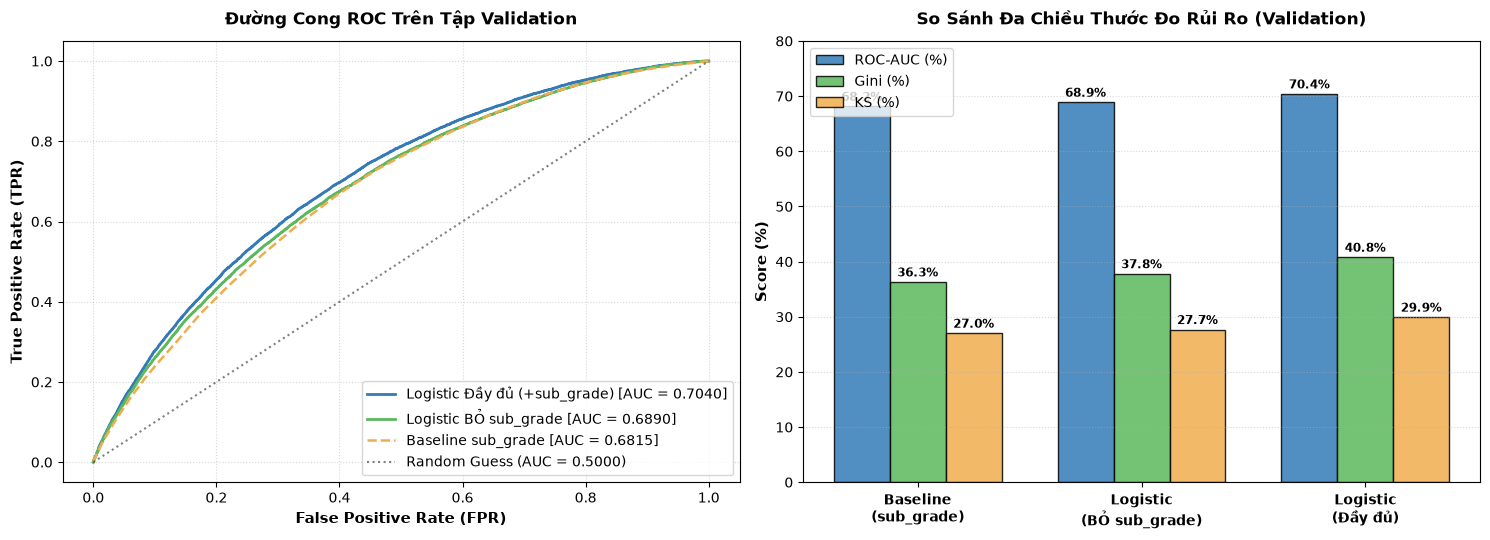
\includegraphics[width=\textwidth]{Images/nosg_roc.png}
\caption{Validation ROC curves (left) and AUC/Gini/KS bars (right) for the baseline, logistic without \code{sub\_grade} and logistic with all features. Axis and legend text are in Vietnamese in the notebook output.}
\label{fig:nosgroc}
\end{figure}

Table~\ref{tab:coef} shows how the coefficients of eight key numeric features change when \code{sub\_grade} is removed. Four coefficients grow by a factor of 1.9 to 2.6: \code{fico\_avg} from $-0.1067$ to $-0.2374$ (2.22$\times$), \code{log\_annual\_inc} from $-0.0386$ to $-0.1021$ (2.64$\times$), \code{inq\_last\_6mths} from $+0.0494$ to $+0.0951$ (1.92$\times$) and \code{revol\_util} from $+0.0521$ to $+0.0978$ (1.88$\times$). Others change little: \code{acc\_open\_past\_24mths} 1.12$\times$, \code{dti} 1.24$\times$, \code{loan\_to\_income} 0.88$\times$ and \code{mort\_acc} 0.98$\times$. This pattern is consistent with \code{sub\_grade} \emph{absorbing} part of the signal that these variables carry: when the grade is available, the model leans on it and gives smaller weights to the variables it partly encodes. It is an association in a fitted model, not a causal statement about how the platform builds the grade. Figure~\ref{fig:coefshift} shows the eight coefficients and the scatter of all 118 shared coefficients.

\begin{table}[H]
\centering
\caption{Standardised logistic coefficients of eight numeric features with and without \code{sub\_grade}.}
\label{tab:coef}
\small
\begin{tabular}{lrrrr}
\toprule
\textbf{Feature} & \textbf{With} & \textbf{Without} & \textbf{Shift} & \textbf{Ratio} \\
\midrule
fico\_avg & $-0.1067$ & $-0.2374$ & $-0.1307$ & 2.22 \\
dti & $+0.1277$ & $+0.1583$ & $+0.0306$ & 1.24 \\
log\_annual\_inc & $-0.0386$ & $-0.1021$ & $-0.0634$ & 2.64 \\
revol\_util & $+0.0521$ & $+0.0978$ & $+0.0457$ & 1.88 \\
inq\_last\_6mths & $+0.0494$ & $+0.0951$ & $+0.0457$ & 1.92 \\
loan\_to\_income & $+0.1491$ & $+0.1310$ & $-0.0181$ & 0.88 \\
acc\_open\_past\_24mths & $+0.1587$ & $+0.1785$ & $+0.0198$ & 1.12 \\
mort\_acc & $-0.0141$ & $-0.0138$ & $+0.0002$ & 0.98 \\
\bottomrule
\end{tabular}
\end{table}

\begin{figure}[H]
\centering
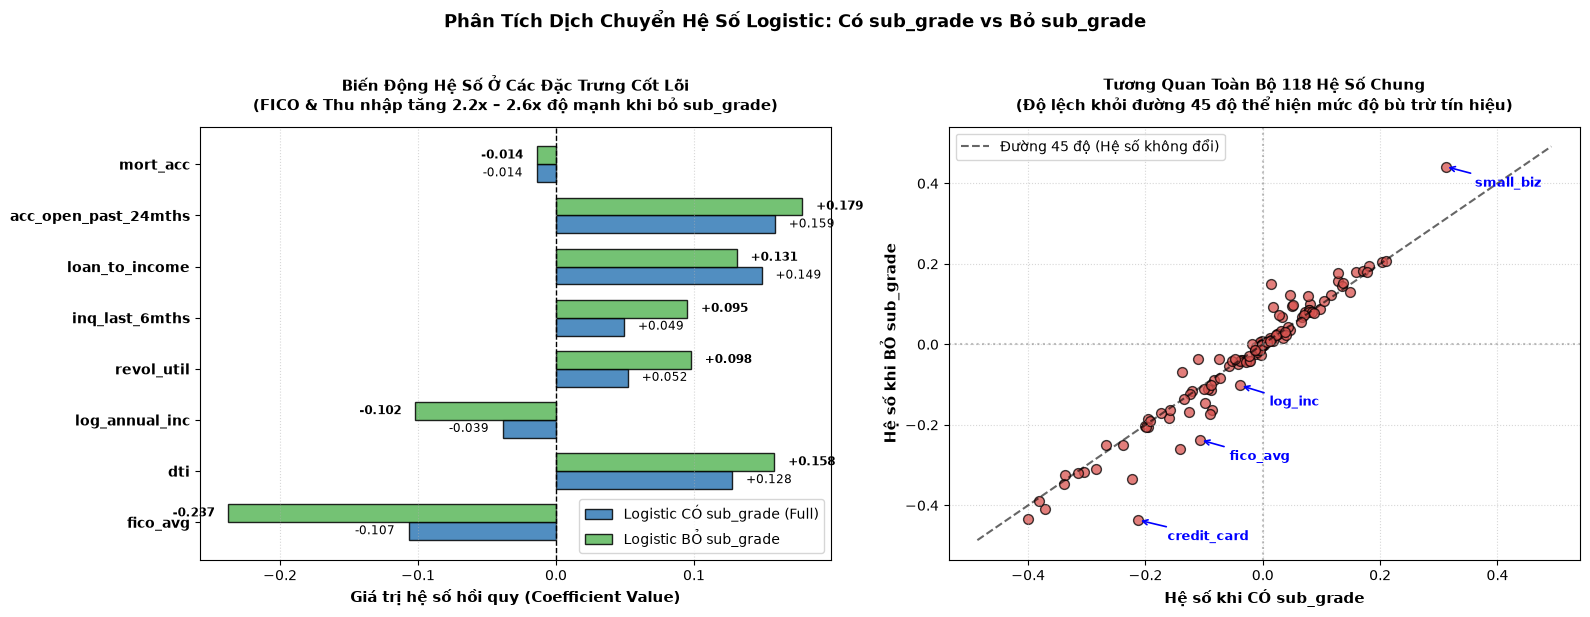
\includegraphics[width=\textwidth]{Images/coef_shift.png}
\caption{Left: coefficients of eight numeric features with and without \code{sub\_grade}. Right: all 118 coefficients present in both models (dashed line: unchanged). Text in the figure is Vietnamese as produced by the notebook.}
\label{fig:coefshift}
\end{figure}

\subsubsection{Experiment 2: compact 12-field scorecard}

The compact model uses 12 fields (30 columns after encoding) and no \code{sub\_grade}. Table~\ref{tab:compact} shows its performance: validation AUC 0.6750 (Gini 34.99\%, KS 25.63\%) and test AUC 0.6730 (Gini 34.60\%, KS 25.07\%). This is \emph{below} the \code{sub\_grade} baseline on both sets ($-0.0066$ on validation, $-0.0088$ on test). Relative to the full 153-feature model, the compact model keeps 84.8\% of the test Gini (34.60\% versus 40.79\%) with 30 instead of 153 columns (about 80\% fewer).

\begin{table}[H]
\centering
\caption{Compact 12-field logistic model versus the full model and the baseline.}
\label{tab:compact}
\small
\begin{tabular}{lcccccc}
\toprule
\textbf{Model} & \textbf{AUC val} & \textbf{Gini val} & \textbf{KS val} & \textbf{AUC test} & \textbf{Gini test} & \textbf{KS test} \\
\midrule
Baseline \code{sub\_grade} & 0.6815 & 36.31\% & 27.02\% & 0.6818 & 36.36\% & 26.45\% \\
Full logistic (153 columns) & 0.7040 & 40.79\% & 29.94\% & 0.7039 & 40.79\% & 29.87\% \\
Compact logistic (30 columns) & 0.6750 & 34.99\% & 25.63\% & 0.6730 & 34.60\% & 25.07\% \\
\bottomrule
\end{tabular}
\end{table}

With $\mathrm{PDO}=20$ and 600 points at default odds 1/5, the validation scores range from 494 to 757 (mean 610.7, median 610; 10th, 50th and 93rd percentiles 588, 610 and 640). Using cut-offs 590, 615 and 640 (chosen from the validation distribution) the four bands behave as in Table~\ref{tab:bands}. On validation the observed default rate falls from 29.38\% in the lowest band to 3.45\% in the highest; on the untouched test set the same cut-offs give 30.18\% and 3.26\%, with intermediate bands 17.28\% and 8.66\%. The ordering and the approximate levels hold out of time. The lowest band holds 11.4\% of test loans and the highest 7.5\%, against an overall test default rate of 14.82\%. Figure~\ref{fig:scorecard} shows the score distributions of repaid and defaulted test loans and the ten numeric weights of the scorecard. The action labels attached to the bands in the notebook (automatic rejection, manual review, \dots) are illustrative; no cost or profit analysis was performed, so we make no claim about their business value.

\begin{table}[H]
\centering
\caption{Score bands of the compact scorecard: share of loans and observed default rate (cut-offs chosen on validation, applied unchanged to test).}
\label{tab:bands}
\small
\begin{tabular}{lrrrrrr}
\toprule
 & \multicolumn{3}{c}{\textbf{Validation}} & \multicolumn{3}{c}{\textbf{Test}} \\
\cmidrule(lr){2-4}\cmidrule(lr){5-7}
\textbf{Band (points)} & Loans & Share & Default & Loans & Share & Default \\
\midrule
$<590$ & 11,279 & 12.2\% & 29.38\% & 10,145 & 11.4\% & 30.18\% \\
590--614 & 44,394 & 47.9\% & 17.08\% & 42,171 & 47.6\% & 17.28\% \\
615--639 & 30,379 & 32.8\% & 8.32\% & 29,671 & 33.5\% & 8.66\% \\
$\ge640$ & 6,579 & 7.1\% & 3.45\% & 6,682 & 7.5\% & 3.26\% \\
\bottomrule
\end{tabular}
\end{table}

\begin{figure}[H]
\centering
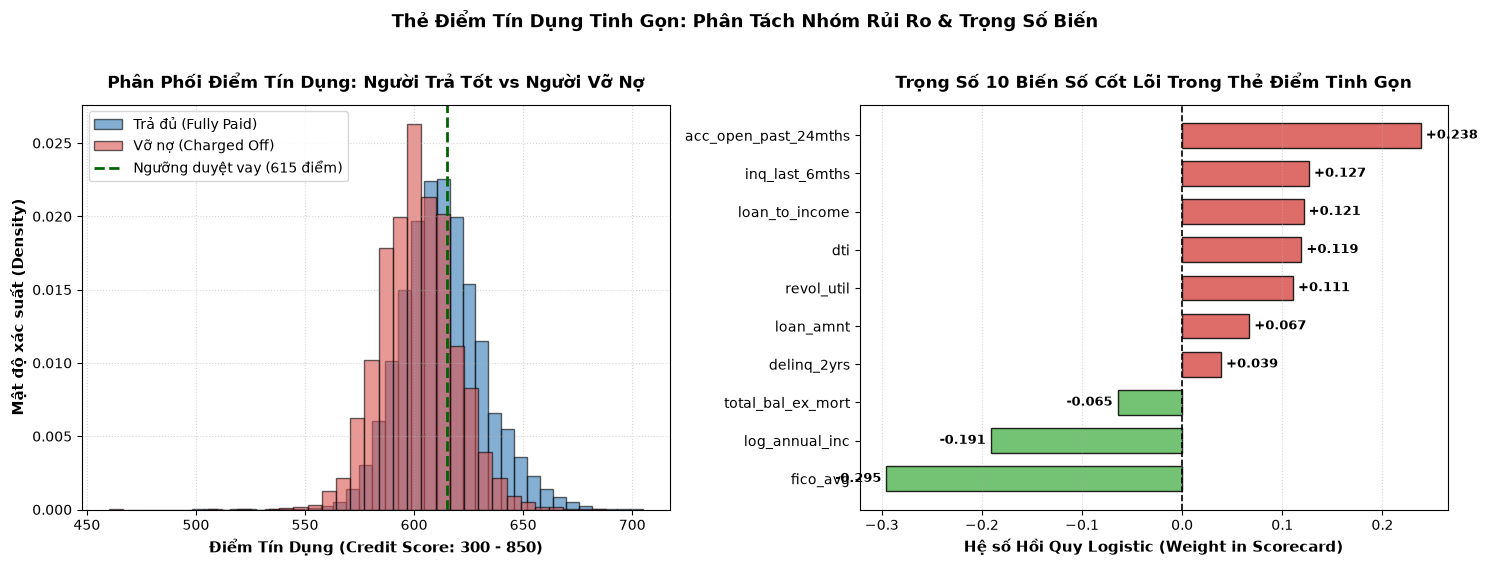
\includegraphics[width=\textwidth]{Images/scorecard.png}
\caption{Left: density of the scorecard points for repaid and defaulted test loans. Right: weights of the ten numeric features in the compact scorecard. Text in the figure is Vietnamese as produced by the notebook.}
\label{fig:scorecard}
\end{figure}

\subsection{Discussion}
\label{sec:res-disc}

\paragraph{Does application-time information beat the incumbent?} Yes, with the grade included: logistic regression and boosting improve test AUC by $+0.022$ to $+0.024$ (Gini by 4.4 to 4.7 points), and the validation intervals exclude zero. Without the grade the other features still beat the grade-based rule, but only by $+0.0061$ AUC on test ($+0.0075$ on validation, CI $[+0.0033,+0.0117]$). Both findings matter: the sub-grade is a strong reference, and what the extra variables add is modest in absolute terms. This ordering is in line with earlier Lending Club work reporting the grade as the most predictive single factor with accuracy improving when other information is added \cite{serrano2015}, but we make no numerical comparison with other studies, since their data, filters and splits differ.

\paragraph{Linear versus non-linear.} Boosting was nominally best (validation AUC 0.7054 versus 0.7040), yet the paired bootstrap interval for the difference $[-0.0002,+0.0031]$ includes zero, and the test values (0.7055 versus 0.7039) differ by 0.0016. The data therefore do not show a benefit of non-linear structure beyond what the regularised linear model already captures, although the decile analysis showed non-monotone behaviour in \code{loan\_amnt}. The random forest was clearly worse than both ($+0.0061$ against the baseline, with the largest overfitting gap), possibly because its tuned grid ended at the edge (depth 10) while the time-ordered CV favoured deeper trees; we did not test this. The single shallow tree was worse than the baseline. Choosing logistic regression is justified by parsimony and interpretability, not by higher accuracy.

\paragraph{Results that did not go the expected way.} (i) The compact 12-field scorecard is below the baseline in AUC, so it is useful only where the platform's grade is unavailable, and even then at a cost of about 0.009 test AUC relative to the grade rule and 0.031 relative to the full model. (ii) The validation AUC of the baseline and of logistic regression is higher than their training AUC, which we cannot explain with the evidence at hand. (iii) The test set confirms the validation conclusions but cannot extend them, because it covers only three months.

\paragraph{Use of the scorecard bands.} The observed default rates in the bands (3.26\% to 30.18\% on test) show that the compact score ranks risk sharply even though its AUC is below the grade; the top and bottom bands are a small share of loans (7.5\% and 11.4\%), so most loans fall in the two middle bands whose default rates (8.66\% and 17.28\%) are close to the overall rate.

\subsection{Limitations and threats to validity}
\label{sec:limits}

\begin{enumerate}
    \item \textbf{Population.} The results apply to accepted, matured, 36-month Lending Club loans issued 2012--2015. Rejected applicants are not in the file, so we cannot say how the models behave on them, and 60-month loans are excluded.
    \item \textbf{Short test window.} The test set covers three months (October--December 2015), and about 0.3\% of December 2015 loans have no final outcome by the snapshot. Conclusions about the stability over longer periods or in other economic conditions are not supported.
    \item \textbf{Temporal drift.} The default rate rises from 13.7\% to 14.8\% across the sets; we did not test or model dataset shift (for example with adversarial validation \cite{qian2021}).
    \item \textbf{Tuning grids at their edges.} The selected random-forest and boosting settings lie on the grid boundary, and neighbouring configurations differ by about 0.001 in CV AUC. Better settings may exist, which could change the random-forest result and possibly the boosting--logistic comparison.
    \item \textbf{Uncertainty quantification.} The bootstrap resamples the validation loans only: it ignores the variability from refitting, from the choice of hyperparameters and from time, it was not repeated on the test set, and a single random seed is used.
    \item \textbf{Test-set use.} The test set is used once for model comparison in notebook~3 and is not used for tuning. The two follow-up notebooks also report test metrics for descriptive purposes after the main selection; they do not change which models are chosen, but the ``single use'' claim applies to the main comparison only.
    \item \textbf{Missing data.} Median imputation is applied to 26 columns that are 5--30\% missing in training, without missing-indicator variables, and five \code{mths\_since\_...} columns were removed for being more than 30\% missing; we did not study whether missingness itself is informative.
    \item \textbf{Probabilities and decisions.} Only ranking metrics are evaluated. Calibration, thresholds, profit and cost trade-offs were not examined; the PDO scaling constants are conventions we did not validate against any standard.
    \item \textbf{Role of \code{sub\_grade}.} \code{sub\_grade} is an application-time variable produced by the platform's own model. Including it makes the problem ``improve on the incumbent''; excluding it (Experiment~1) makes it ``replace the incumbent''. Both are reported, but the decision of which to use in practice depends on the use case.
    \item \textbf{Fairness and geography.} The models use \code{addr\_state} and \code{home\_ownership}; we did not analyse whether they create disparate impact.
    \item \textbf{Single dataset.} No external dataset was used for validation.
\end{enumerate}

\subsection{Chapter summary}

On 589,488 matured 36-month loans split by time, logistic regression and histogram gradient boosting improve the out-of-time AUC over the sub-grade baseline by about 0.022--0.024 (test AUC 0.7039 and 0.7055 versus 0.6818), with bootstrap intervals that exclude zero, and they are statistically indistinguishable from each other; the random forest improves less, and a single tree does worse than the baseline. Without \code{sub\_grade}, logistic regression still beats the baseline but only by 0.0061 on test, and the weights of FICO, income, inquiries and utilisation roughly double. A compact 12-field scorecard falls below the baseline yet separates risk bands from 3.26\% to 30.18\% observed default. The limitations include a short test window, grid-edge tuning, validation-only bootstrap intervals and an unexplained validation-above-training AUC for two models.
